\section{Simulator in C++}
This is another simulator for the same kind of experiment.
Again, the robot moves and, when the landmark is in range, the robot detects the relative bearing.

It has been developed in C++, and uses the SFML libraries.

This simulator is simpler than the previous one, to the cost of a coarser approach to errors.
Noise is simply modeled as uniformly distributed between two values, while in the Matlab simulator a gaussian distribution was used (see section \ref{sec:matlab_simulator} for details).

\begin{figure}[htbp]
  \centering
    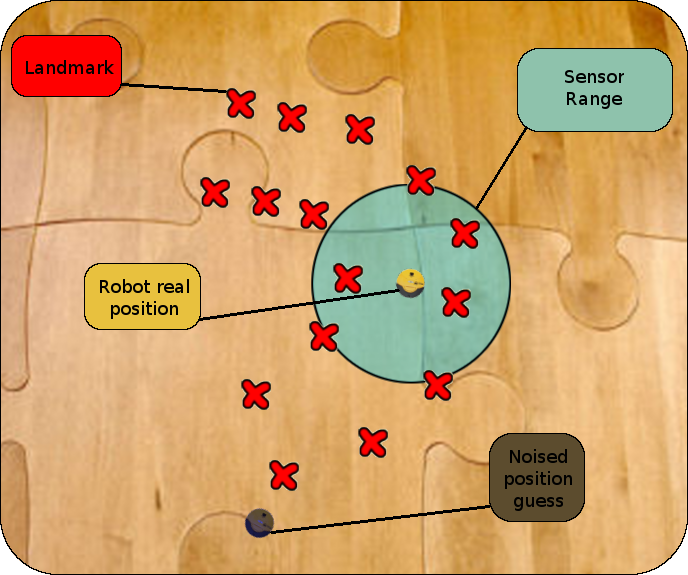
\includegraphics[width=0.6\textwidth]{images/cpp_simulator.png}
  \caption{Part of a screenshot of the C++ simulator. Elements have been labeled.}
  \label{fig:cpp_simulator}
\end{figure}

The user can move the robot, resize the sensor range and add landmarks.

This program outputs two files: the first one contains the ``real'' odometry and measurements, while the other one contains the ``noised version'' of the same data.

